% !TeX root = ../main.tex

\chapter{区块链技术}

\section{区块链系统简介}

区块链技术旨在不可信的开放网络中,维护一个安全可信、不可篡改的公共账本,并以此为基础构建电子 交易、访问控制等应用系统.根据新节点的加入是否需要授权认证,区块链系统可以分为许可链和非许可链两 大类.非许可链通常也称为公有链,不限制节点的加入或退出,任何节点可以访问链上数据、发布交易、以及 参与链上数据的记录,甚至可以尝试发布不合法消息,攻击网络中的其他节点.许可链指区块链网络中节点 的加入网络、记录账本等操作需要经过特定的授权许可与认证.许可链系统又可以根据系统参与方的数量分 为联盟链与私有链,其中联盟链由多方组织加入同一区块链网络中,共同维护区块链账本,记录并执行链上合 约,多方组织可以通过一致的账本建立起联盟成员之间的信任.而私有链通常由一个参与方负责创建和维护, 主要用于记录和管理内部数据,增强数据的安全性、可追溯性. 

本文对比许可链和非许可链两类区块链系统在准入限制、参与方数量、采用的共识算法、应用场景等方面的区别,并总结如表\ref{tab:classification} 所示. 

\begin{table}[htb]
  \centering
  \begin{minipage}[t]{1\linewidth} % 如果想在表格中使用脚注,minipage是个不错的办法
  \caption[模板文件]{区块链系统分类}
  \label{tab:classification}
    \begin{tabularx}{\linewidth}{lXX}
      \toprule[1.5pt]
      {\heiti 名称} & {\heiti 非许可链} & {\heiti 许可链} \\\midrule[1pt]
		准入限制  & 无准入限制,任意节点可以随时加入或者退出 & 有准入限制,准入限制由整个联盟的节点商议后制定 \\
		参与方数量  & 较多 & 较少 \\  
		共识算法  & POW, POS等共识算法 & BFT类分布式共识算法 \\  
		区块链性能  & 较低 & 较少 \\  
		应用场景	 & 密码货币交易系统 & 公司间合同,公司内事务管理 \\  
		典型应用  & Bitcoin, Ethereum & HyperLedger, Coco \\
      \bottomrule[1.5pt]
    \end{tabularx}
  \end{minipage}
\end{table}

\section{密码学基础}

区块链系统中引入大量的密码学技术提供安全性、可信性等密码学性质,并以此作为区块链价值的底层保障。目前主要有哈希算法、非对称加密体制、电子签名、布尔集合、密码累加器、同态加密、零知识证明、安全多方计算等密码学技术用于区块链系统。本章主要介绍广泛应用的哈希算法,非对称加密,电子签名和布尔过滤器。

\subsection{哈希函数}

哈希函数,通常也称散列函数,是一种将任意长度的输入转换为固定长度的输出的函数。哈希函数的表示形式为:
$$h=H(m)$$
其中,m为任意长度消息,H为哈希函数,h为固定长度的哈希值,通常也称为消息摘要。

哈希函数具有如下特性:
\begin{enumerate}
\item 单向性:从输入计算输出很简单,但在不知道输入的情况下,通过输出计算出输入是计算上不可行的;
\item 输出的随机性:即算法输出的每一位数据在统计学意义上都符合随机分布;
\item 雪崩效应:对输入的任何一点修改,都会导致输出的大量变化;
\item 抗碰撞性:找到两个具有相同的输出的不同输入,是计算上不可行的。
\end{enumerate}

正是由于上述重要特性,哈希算法被广泛应用于消息认证码、随机数产生、错误校正与检测等领域,而在区块链系统中,哈希算法主要用于检查数据是否被篡改,提供工作量证明,构造存在性证明这几个用途。传统互联网中,哈希算法常用于数据的完整性验证。为了验证互联网中的文件在传输过程中是否被篡改,通常采用存储验证文件哈希值的方式,利用了哈希函数的雪崩效应和抗碰撞性,一旦数据被篡改,最终的哈希值一定与之前存储的哈希值不同。而在区块链系统中,由于交易数据不断增长,账户状态不断变化,如果采用全部数据求哈希值的方法,则每次改变都需要重新计算哈希值,计算复杂度不可接受。因此,在区块链系统中,数据根据时间顺序组织成了若干个区块,一定时间内新发生的事务数据存储在一个新区块里,每一个区块都包含了上一个区块的哈希值。这样的数据组织方式如同区块形成的链状结构,因而称为区块链。具体组织结构如图\ref{fig:hashchain}所示。


\begin{figure}
\centering	
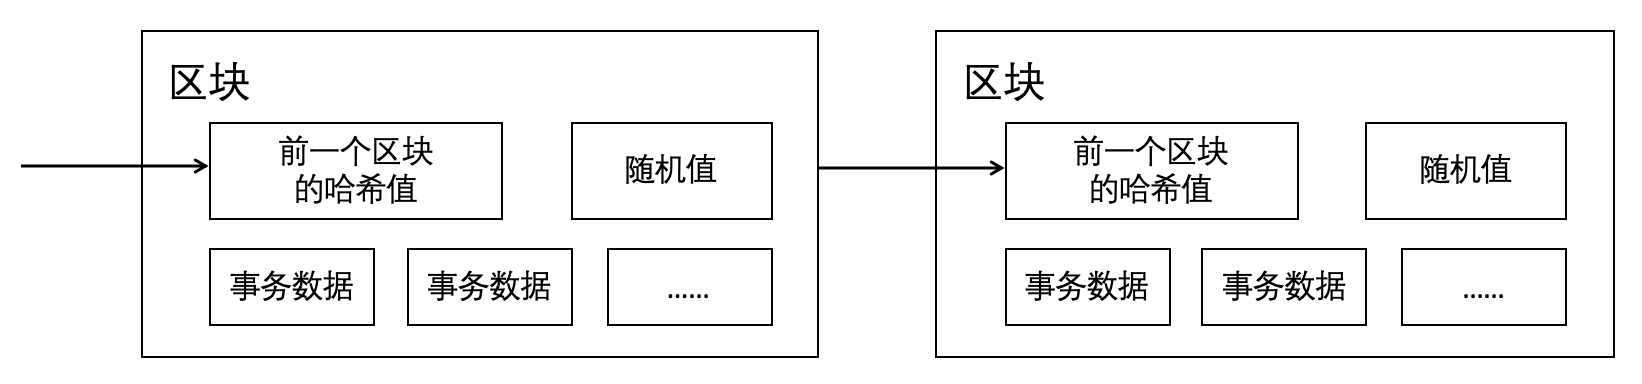
\includegraphics [width=400pt,height=100pt]{figures/hashchain.png}
\caption{区块链数据结构}
\label{fig:hashchain}
\end{figure}

如果区块链中任意区块里的数据被篡改,那么该区块的哈希值与后一区块记录的哈希值不相等。由哈希函数的雪崩效应可知,区块链上的任何历史数据改动都能被检测。因此,节点只需要存储最新区块的哈希值,即可通过计算检验历史上所有区块中的数据是否被篡改。

\begin{figure}
\centering	
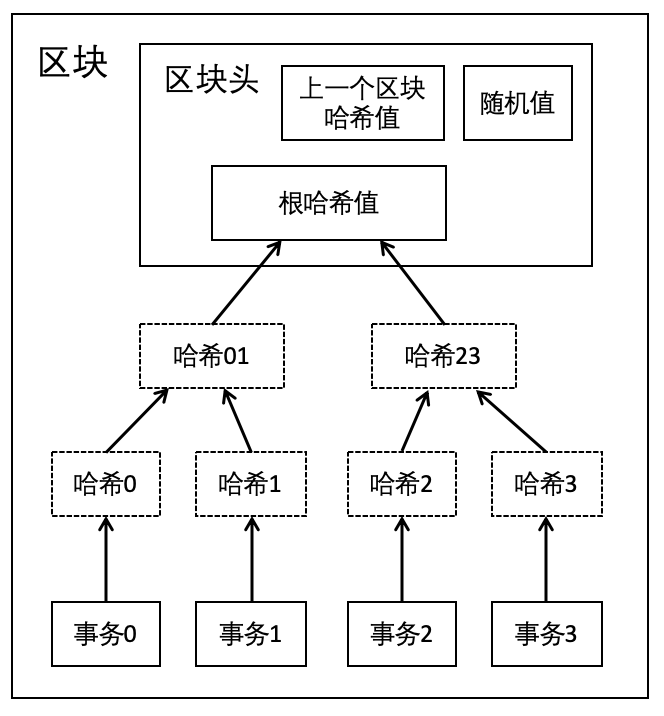
\includegraphics [width=150pt,height=180pt]{figures/merkle-tree.png}
\caption{默克尔树数据结构}
\label{fig:merkle-tree}
\end{figure}

而在每个区块中,哈希函数用于构建默克尔树,即哈希二叉树。如图\ref{fig:merkle-tree}所示,所有事务的哈希值通过二叉树结构进行哈希计算,最终计算得到根哈希值。该数据结构保证,任意事务数据的修改,都会影响到根哈希值。因此区块头中只需要存储根哈希值,就可以验证该区块中所有事务是否被篡改。


\begin{figure}
\centering	
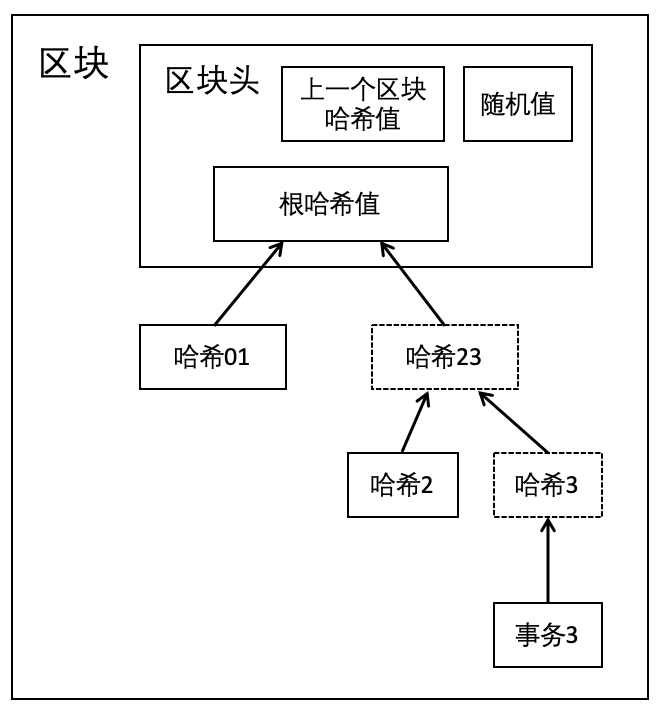
\includegraphics [width=150pt,height=180pt]{figures/merkle-proof.png}
\caption{交易存在性证明}
\label{fig:merkle-proof}
\end{figure}

当用户需要通过根哈希值验证某事务是否在某区块中时,不需要验证该区块中所有事务数据,只需要由存储所有数据的节点提供该事务到根哈希值的路径上所有相关数据。如图\ref{fig:merkle-proof}所示,当用户希望验证事务3是否存储在区块中,只需要验证“事务3”,“哈希2”,“哈希01”这几个数据是否能通过哈希函数得到根哈希值。由哈希函数的抗碰撞性可以保证,证明节点不能提供虚假数据计算出同样的根哈希值。

\subsection{非对称密码体制和电子签名}

密码体制主要分为对称密码体制和非对称密码体制。简单来说,对称密码体制指加密算法中使用的加密密钥和解密算法中使用的解密密钥是相同的密钥,或者解密密钥能通过加密密钥计算得到。而非对称密码体制中,这两者不同,并且解密密钥不能通过加密密钥计算得到。

\begin{figure}
\centering	
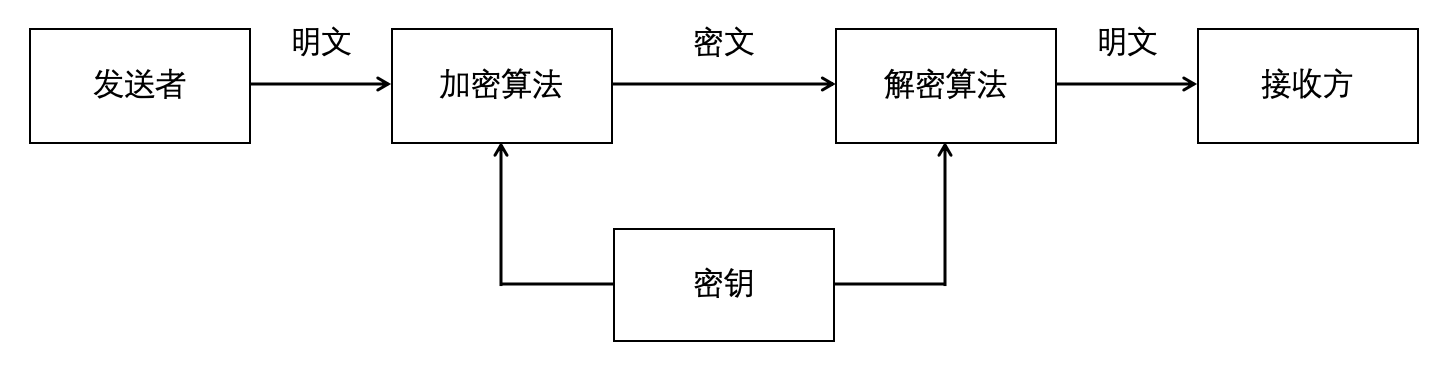
\includegraphics [width=400pt,height=100pt]{figures/sym-crypto.png}
\caption{对称密码体制的基本模型}
\label{fig:sym-crypto}
\end{figure}

如图\ref{fig:sym-crypto}所示,对称密码体制中,发送者先使用密钥和加密算法将明文加密为密文,然后传输密文给接收方,接收方使用解密算法和相同的密钥将密文解密回原始的明文。因为加密和解密算法使用的密钥需要相同,消息发送方和接收方必须在密文传输前通过安全信道进行密钥传输。因此对称密码体制面临密钥分配问题,目前主要通过通信双方直接进行密钥传输或者密钥分配中心进行密钥分发进行。然而实际的传输信道安全性并不理想,密钥在传输过程中被暴露的风险很大,增加了系统的脆弱性。另一方面,在有多个用户的网络中,任何两个用户之间都需要共享加密密钥。当网络中用户$n$很大时,需要管理的密钥数目为$C_n^2$,复杂度近似O($n^2$)。当有一个新用户加入时,需要产生$n$个秘密的密钥,并秘密分发给$n$个用户。对称密码体制中使用的加密算法主要采用扩散和混淆两种基本方法,可以抵抗密码分析技术对密文进行统计分析。扩散指让明文中的每一位尽可能多影响密文中的若干位,以及让密文中的每一位受到明文中尽可能多位的影响,这样可以隐蔽明文的统计特性。字符到字符的映射,通常包含单字符置换和多字符置换。混淆指混淆密文与密钥之间的统计关系,使得对手即使获取了关于密文的一些统计特性,也无法推测密钥。通常使用复杂的非线性代替变换可以达到比较好的混淆效果。

\begin{figure}
\centering	
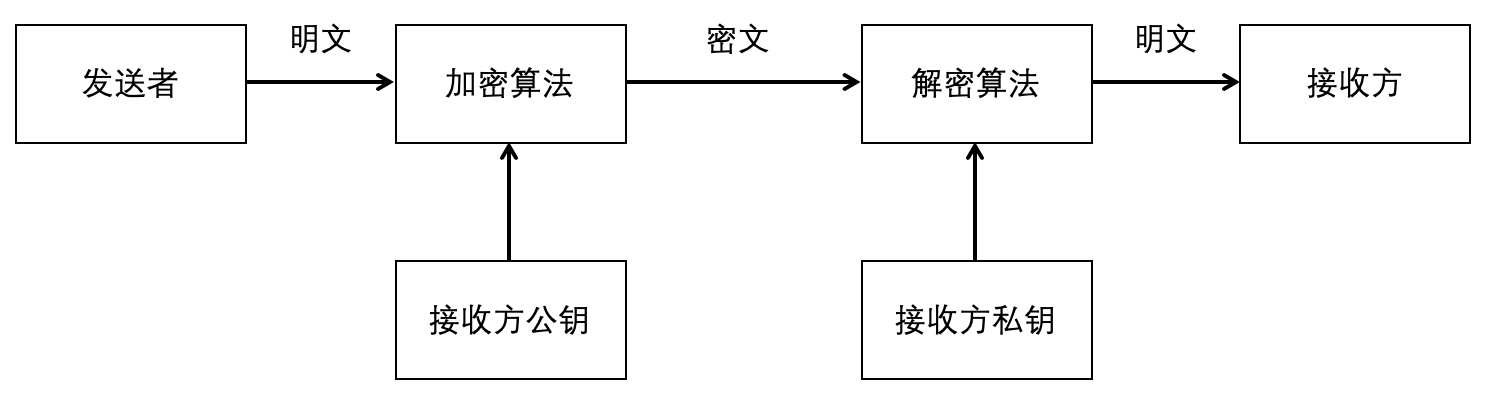
\includegraphics [width=400pt,height=115pt]{figures/asym-crypto.png}
\caption{非对称密码体制的基本模型}
\label{fig:asym-crypto}
\end{figure}

1976年,W.Diffie和M.Hellman在IEEE Trans.on Information刊物上发表了“ New Direction in Cryptography”文章,提出了“非对称密码体制“的概念,开创了密码学研究的新方向。如图\ref{fig:asym-crypto}所示,非对称密码体制中,密钥分为成对的加密密钥和解密密钥,其中加密密钥公开,解密密钥保密。公开的密钥可以作为用户的个人身份,由公开的加密密钥无法推导相应的解密密钥。因此即使将加密密钥公开也不会暴露解密密钥,不会损害密码的安全。因此,通信双方可以通过不安全的信道交换公钥,然后用对方的公钥对消息进行加密并传输,达到在不安全的信道上保密传输的效果。解决了对称密码体制中需要安全信道的问题,同时在密钥管理上也极大降低了网络中需要管理的密钥数量,从对称密码体制的$C_n^2$降低到$n$。对称密码体制与非对称密码体制在密钥分发、密钥管理等方面的区别主要如表\ref{tab:sym-asym}所示。

\begin{table}[htb]
  \centering
  \begin{minipage}[t]{1\linewidth}
  \caption{对称密码体制与非对称密码体制的区别}
  \label{tab:sym-asym}
    \begin{tabularx}{\linewidth}{lXX}
      \toprule[1.5pt]
      {\heiti 功能} & {\heiti 对称密码体制} & {\heiti 非对称密码体制} \\\midrule[1pt]
		密钥分发  & 需要事先进行安全的密钥分发 & 不需要事先进行安全的密钥分发,公钥可以在不安全的信道上传输 \\
		密钥管理  & 每个用户需要保存n个不同密钥用于与其他n个用户通信。当有新用户加入时,每个用户都需要和新用户共享一个新密钥,整个系统中需要存储O($n^2$)个密钥 & 每个用户只需要存储自己的公钥和私钥,整个系统中只需要存储O(n)个密钥 \\
		电子签名  & 不支持电子签名功能 & 支持电子签名功能 \\  
		性能  & 加密算法和解密算法简单,加解密速度较快 & 加密算法和解密算法需要进行复杂的数学运算,速度较慢 \\  
		安全性  & 安全性来源于混淆和置换 & 安全性通常基于数学难问题,部分假设未证明 \\ 
      \bottomrule[1.5pt]
    \end{tabularx}
  \end{minipage}
\end{table}

数字签名,通常也称为电子签名,指通过数据处理的方式对数字消息进行签名。同样具有手写签名的两大特性:可验证性和防伪造性。具体来说,数字签名需要具备以下特性:

\begin{enumerate}
 \item 任何人可以验证数字签名是否由消息的发送方生成。
 \item 任何人不能伪造发送方的数字签名,这也意味着发送方不能抵赖自己生成的数字签名。
 \item 任何人可以验证数字签名是否匹配发送的消息,因此可以验证消息从发送到接受过程中是否被篡改。对整个消息生成数字签名过于复杂,因此通常先对消息计算哈希值,然后生成哈希值的数字签名用于验证。
\end{enumerate}

某种意义上,我们可以认为数字签名的过程是一种加密,而对签名还原到原消息,然后进行验证是一种解密。但与非对称公钥体系中的公钥加密,私钥解密恰好相反,通过私钥计算签名,然通过公钥进行验证。由于公钥公开,因此所有人可以知道该公钥的持有者。而只有该用户拥有对应的私钥,才能生成正确的数字签名。

在区块链领域,每个用户都可以通过特定算法独立生成任意多账户,即公私钥对。当用户发起事务时,需要用私钥生成事务数据的电子签名。当该事务涉及其他用户时,使用特定用户公钥生成的地址。

\subsection{布尔过滤器}

为了验证某数据是否存在集合中,传统算法主要有遍历查找,二分查找,索引查找等,这些算法的时间消耗都会随着集合数量的增加而增加。为了解决这一问题,布尔过滤器利用哈希算法的输出长度固定性和随机性,利用固定长度的数组存储集合,对元素进行哈希变换,然后根据输出找到对应下标并在数组中记录或查询。为了解决不同输入映射到同一下标的问题,通常采用多个哈希函数共同确认。布尔过滤器具有很好的空间和时间效率,被用来检测一个元素是不是集合中的一个成员。在以太坊项目中,布尔过滤器被用于检测交易是否在给定区块中,便于用户快速检索特定交易的存储位置。和布尔过滤器类似,密码累加器也用于高效验证数据的存在性,后者还可以提供高效安全的存在性证明。在零币项目中,密码累加器用于存储用户加入的未花费代币的对应编码,当用户使用时,其他用户可以高效验证花费的代币是否存在。

\section{共识协议}

多个节点为了达成关于某些数据的同步,需要共同运行的共识协议进行保障。在传统的分布式领域,例如分布式数据库,所有节点由同一公司或者组织运行,因此各节点的安全性、可信性都能得到保障,主要需要考虑的是节点出现共识模块关闭、消息网络延迟、节点宕机等异常情况。而攻击者入侵控制系统中某些节点,则可以通过发送错误数据破坏节点间的共识。这类被入侵节点被称为拜占庭节点,来源于一篇论文中提到的拜占庭将军进攻罗马的故事。因此,一类能抵抗拜占庭节点的共识协议提出,被称为拜占庭容错共识协议。传统的分布式共识协议,包括拜占庭容错共识协议和非拜占庭容错共识协议,都是基于可信身份的投票机制。各节点明确知道当前共识系统中的节点数量以及各节点公钥,可以验证信息来源于某一节点。而在区块链领域中,为了达到去中心化的目的,节点不受某一公司或者组织管理,可以自由加入和退出。如果采用传统的分布式共识协议,通过基于身份的投票达成共识,攻击者可以构建任意多的身份参与投票,也就是采取女巫攻击。因此,在公有链领域需要采用无身份的共识,目前主要采用工作量证明共识协议。

\subsection{传统分布式共识协议}
\label{subsec:traditional-consensus}

传统分布式共识协议主要根据能否抵抗拜占庭节点,分为拜占庭容错共识协议和非拜占庭容错共识协议两类。本节主要介绍非拜占庭容错共识协议Paxos和Raft,以及拜占庭容错共识协议PBFT。

Leslie Lamport于1989年首次发布Paxos协议,并以论文中希腊Paxos岛上使用的一个虚构的立法共识系统命名。这篇文章后来在1998年以期刊文章的形式发表。Paxos通过处理器在协议中的角色来描述处理器的动作:客户端、接受者、提议者、学习者和领导者。在典型的实现中,单个节点可能同时扮演一个或多个角色。这并不影响协议的正确性——通常合并角色来改进协议中的延迟和/或消息数量。

\begin{description}
  \item[客户端] 客户端向分布式系统发出请求,并等待响应。例如,对分布式文件服务器中的文件的读/写请求。
  \item[接收方(选民)] 接受方充当协议的容错“存储器”,接收方集合称为Quorums。发送给接收方的任何消息必须发送到接收方全体集合。从接收方接收到的任何消息都将被忽略,除非从集合中的每个接收方接收到相同的消息。
  \item[提案方] 提案方主张客户端请求,试图说服接收方同意它,并充当协调者,在冲突发生时推动协议继续,保障共识的活性。
  \item[学习方] 学习方充当协议的备份节点。一旦接收方同意了客户端的请求,学习者就可以采取行动执行请求并向客户端发送响应。为了提高系统的可用性,可以添加额外的学习者。
  \item[领导方] 系统达成一致需要领导方的提案并且协同。许多节点可能同时认为自己是领导者,但协议只保证在最终选出一个领导方时才能继续。如果两个节点都认为它们是领导方,可能会通过不断提出相互冲突的更新来阻止协议。然而,在这种情况下,仍能保障系统安全性。
\end{description}

一轮成功的Paxos共识从分布式系统中某节点接收到客户端发起的请求开始,到系统对该请求达成一致性结果结束。主要分为提议和接受两个阶段,每个阶段各包含两个步骤。

\begin{description}
  \item[提议阶段] 提议阶段包含准备和承诺两个阶段
  \begin{enumerate}
    \item 准备:收到客户端请求的节点充当提案方创建一个消息,我们称之为“准备”,它的编号为数字$n$。$n$不是要提议的值,它只是由提案方(发送给接收方)唯一标识这个初始消息的数字。编号$n$必须大于此提案方在先前的任何“准备”消息中所使用的编号。然后,它将包含$n$的“准备”消息发送给接收方集合。“准备”消息只包含数字n,不包含客户端发送的请求信息。
    \item 承诺:任何接收方都在等待来自任何提案方的“准备”消息。如果接收方收到一条“准备”消息,接收方检查编号$n$。如果$n$大于此前从任意提案方接受的所有提案编号,接受方必须返回一个“承诺”消息给提案方,并且忽略此后接收到的所有编号小于$n$的“准备”消息。如果接收方此前已接受某提案,则需要将包含接受的提案编号$m$和对应的值$w$的“提案”消息返回给提案方。
否则,如果n小于或等于接收方此前从任何提案方收到的提案编号,接收方可以忽略所收到的提案。
  \end{enumerate}

  \item[接受阶段] 提议阶段包含准备和承诺两个阶段
  \begin{enumerate}
    \item 接受请求:如果提案方收到来自大多数接收方集合的“承诺”消息,则需要为其“提案”消息设置一个值$v$,通常这个值表示从客户端接收到的请求数据。如果任何接收方曾经接受过提议,在提议阶段的承诺步骤中,会将接受的“提案”消息返回给提案方。提案方从接收到的所有“提案”消息中找出最大编号的提案,假设该提案的值为$z$,则需要将“提案”消息的值设为$z$。如果没有一个接收方返回“提案”消息,那么提案方可以选择自己的提案值$x$。提案者在选定值后,向接收方集合发送一个“接受”消息,包含编号$n$和提案值$v$,其中编号$n$与此前的“准备”消息一致。
    \item 接受:当接受者从提议者那里收到一条“接受”消息($n,v$),如果该节点已在提议阶段的承诺步骤中发出承诺只考虑编号大于$n$的提案时,则拒绝该消息。如果接收方尚未承诺,则该节点记录“接受”消息中的值$v$作为接受值。并将“接受”消息发送到提案方和每一个学习方。一个接受者可以接受多个提议,这可能发生在另一个提案方不知道正在决定的新值,并用更大的编号$m$开始新一轮。在这种情况下,接受者仍可以承诺并稍后接受新提议的值。这些提案可能导致接收方集合记录不同的值。然而,Paxos协议将保证接受方最终会同意某一相同的值。
  \end{enumerate}
\end{description}

由于Paxos共识协议的理论和工程实现较为复杂,2014年,Ongaro等人提出了Raft共识协议,简化Paxos共识协议的流程,同时保障了共识的安全性。相较于Paxos共识协议中各节点可以随时充当领导方发起提案,Raft协议中通过领导选举推选出一个固定的节点担任领导方,当该节点故障时再做更换,这一机制减少了冲突出现的可能。因此,在Raft协议中主要包含领导方,追随者和候选人三种角色。

\begin{description}
  \item[领导方] 领导方负责将记录备份给所有追随者,也需要不断发送心跳信息给追随者表明自己处于正常运行的状态。
  \item[追随者] 追随者负责接收并记录领导方发送的消息,同时通过心跳信息监听领导方的运行情况,一旦出现宕机等情况则转为候选人角色。
  \item[候选人] 当追随者发现领导方出现宕机等故障,将进入候选人角色,发起领导选举。
\end{description}

对于Raft协议而言,最重要的是领导选举和记录备份两个部分,

\begin{description}
  \item[领导选举] 当系统开始运行Raft共识协议或者当现有的领导方出现故障时,所有参与节点需要选出一个新的领导方。系统共识的每一轮周期可能持续任意长的时间,都从领导选举开始。如果成功选出领导方,则本轮周期由该领导方负责后续的步骤,直到该领导方出现宕机等故障结束。如果选举失败,则开始新一轮周期,重新选举领导方。

  每轮领导选举由候选人发起。如果在周期$n$中,某节点在一段时间内没有收到领导者的心跳信息,那么该节点将成为候选人,因此它假定当前没有正常运行的领导方。它通过增加周期的计数器,表示进入下一轮周期$n+1$,同时并向所有其他节点发送消息请求它们投票。如果该节点收集到超过一半的投票,则表示该节点成为新的领导方。如果在投票过程中,候选人节点接收到别的节点发出的消息,并且消息包含的周期值不低于当前周期值$n+1$,则该节点停止选举并转为追随者。每个节点在每轮周期中只会进行一次投票,采用先到先得的方式。因此如果多个候选人同时请求投票,则可能所有候选人都收集不到超过一半的投票。在进入候选的时候,每个候选人会启动一个随机的定时器,当定时器到时该节点会增加周期值,进入下一轮周期,再次发起投票请求。由于每个候选人的定时器是随机的,因此可以快速结束分裂投票的状态,选出单个领导方。并由该领导方向其他节点发送心跳信息,保障其他节点停止领导选举。
  \item[记录备份] 在选出领导后,领导方需要负责记录的备份。该领导方接受客户端发送的请求,每个请求包含一条指令,需要集群中每个节点运行。当请求作为一个新条目添加到领导方的日志之后,每个请求都作为“新增条目”消息转发给追随者。如果追随者出现宕机等情况不可用,领导方将不断地重新发送“新增条目”消息,直到日志条目最终被所有追随者存储。这一机制可以保障某些节点宕机重启后,可以再次接收到宕机期间新增的条目,保障了所有节点日志的一致性。一旦领导方从大多数追随者收到条目已经被复制的确认,领导方会将该条目应用于本地的状态机,该请求处于“承诺”状态。同时也会提交领导方的日志中存在的所有条目。一旦追随者得知日志条目处于“承诺”状态,它就会将该条目应用到其本地状态机。这确保了集群中所有服务器之间日志的一致性以及日志同步的安全规则。

  在领导方出现故障,需要选举新的领导方时,日志可能出现不一致的状态,来自旧领导方的部分日志没有在集群中完全复制。因此,新的领导方将通过强制追随者复制自己的日志来处理这一不一致的状态。该机制将从集群故障状态恢复日志一致性。
\end{description}

Paxos共识协议和Raft共识协议只能解决节点宕机和网络通信等故障异常,不能抵抗拜占庭节点的攻击,包括故意构造的错误数据,以及对系统中不同节点发送不同的信息导致系统的不一致。实用的拜占庭容错(PBFT,Practical Byzantine Fault Tolerance)共识协议于1999年提出,能抵抗拜占庭攻击。同时减少了此前拜占庭容错共识协议的时间和通信复杂度,能运用于现实场景。与Raft共识协议类似,PBFT共识协议同样包括“领导方”和“追随者”,这里“领导方”称为“主节点”,“追随者”称为“从节点”。简单而言,PBFT协议的一次正常共识过程分为以下五个阶段:

\begin{figure}
\centering  
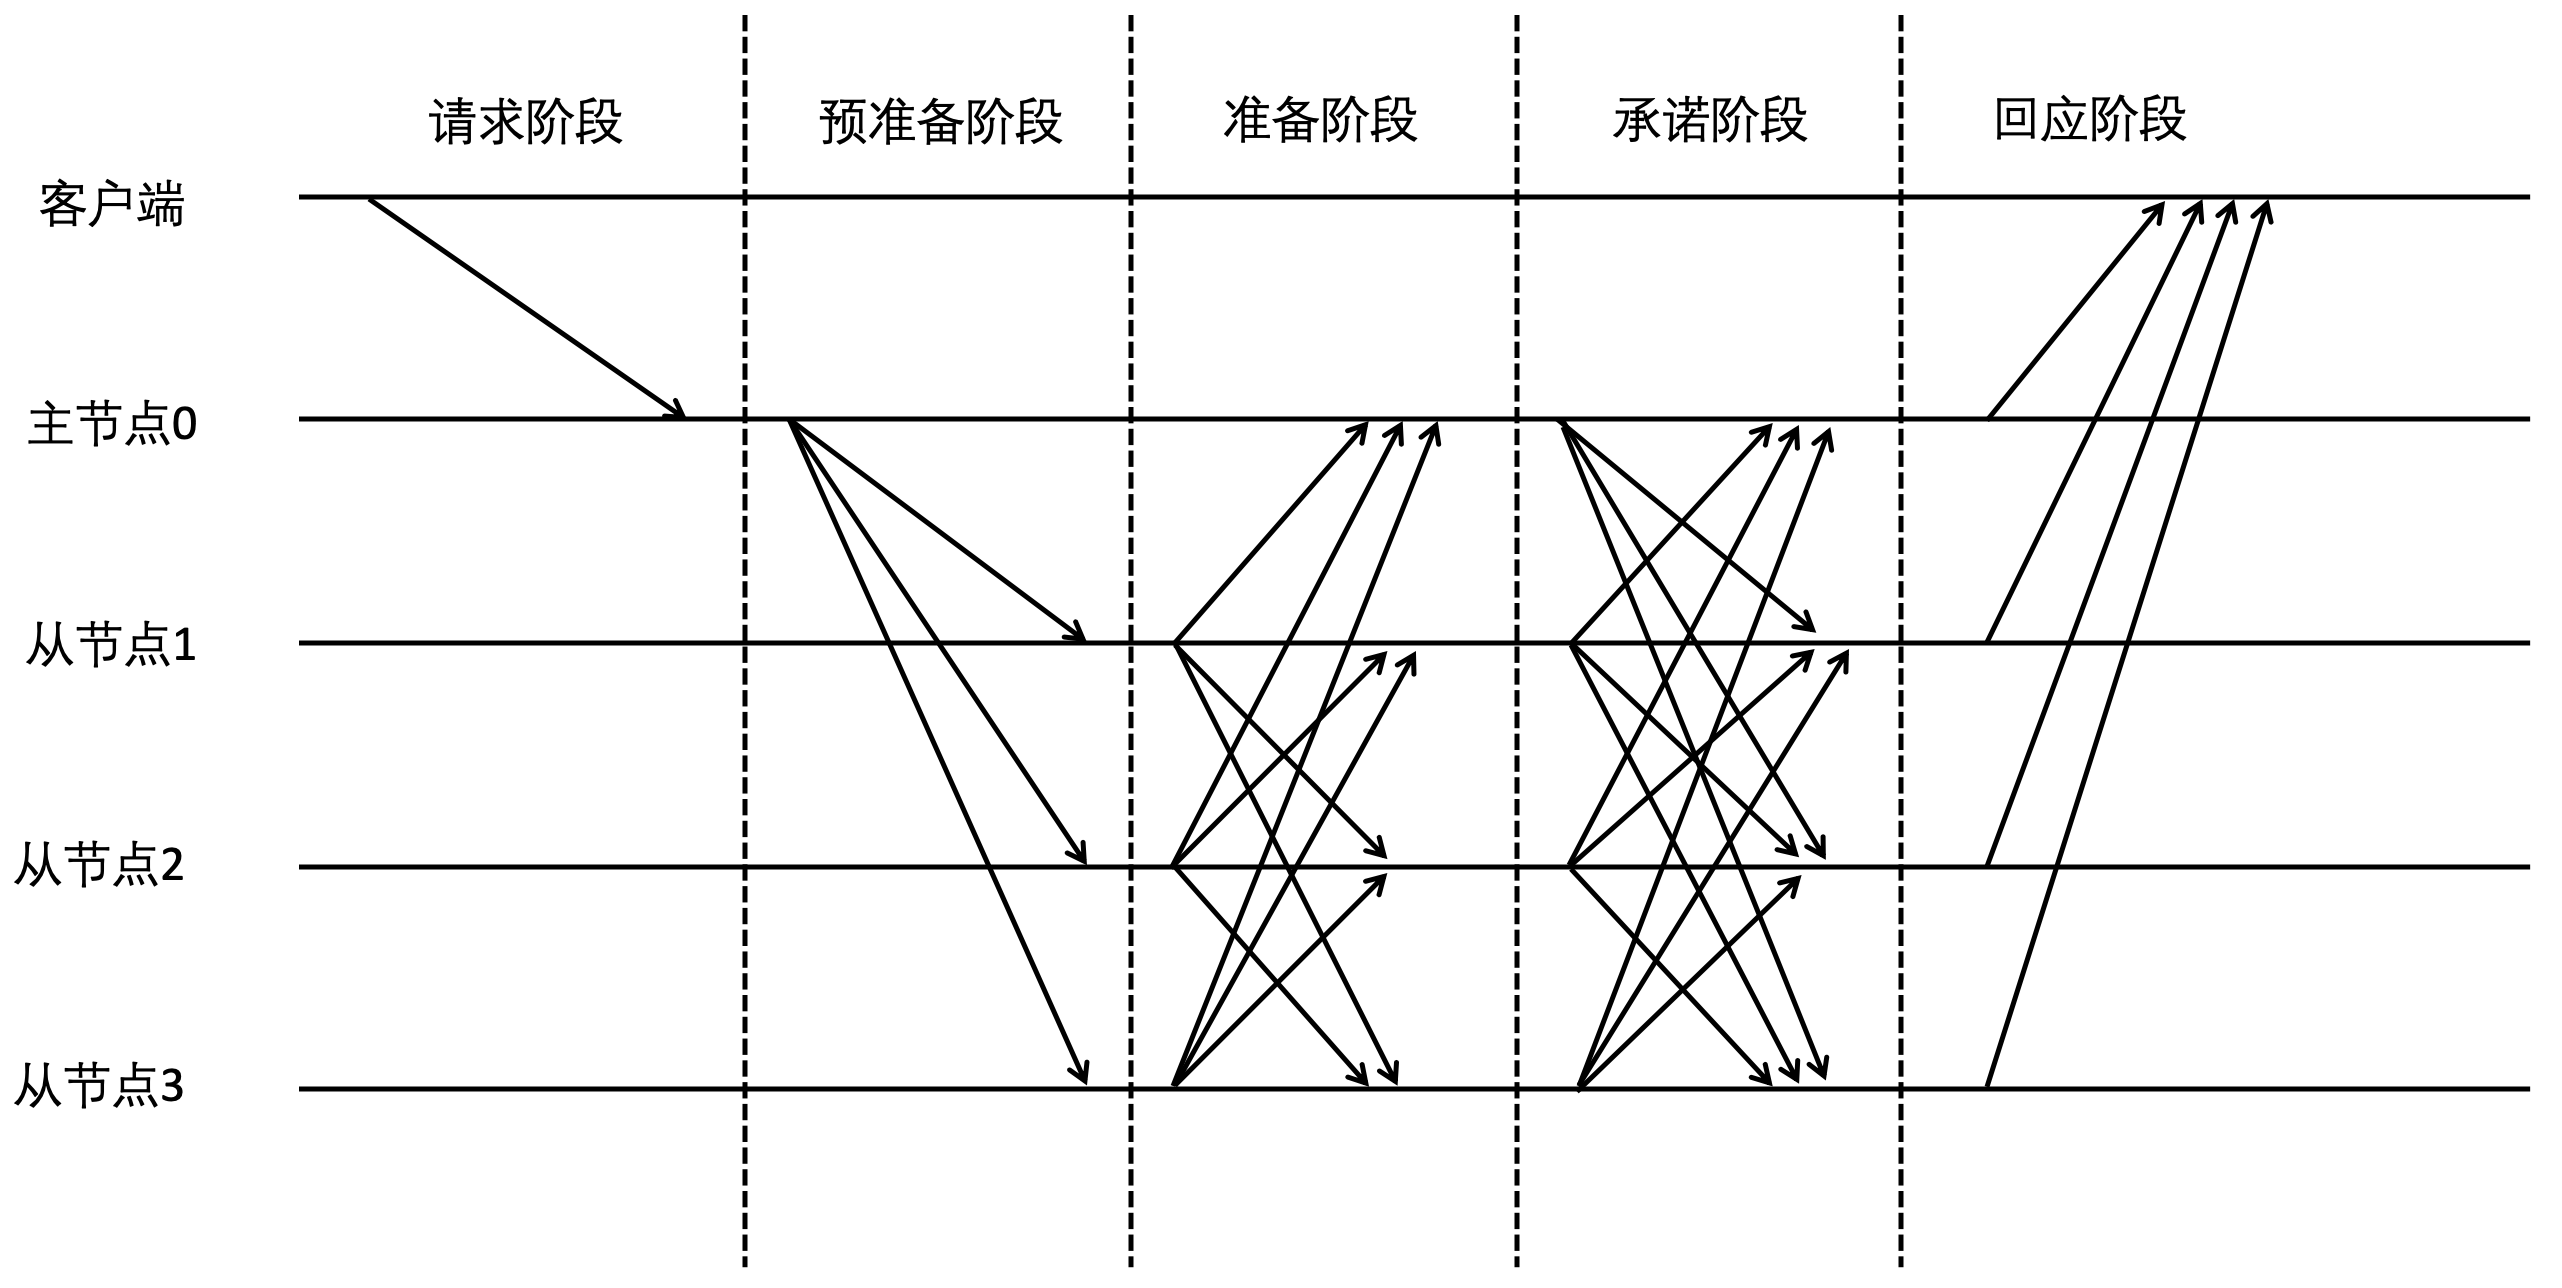
\includegraphics [width=400pt]{figures/pbft.png}
\caption{PBFT共识协议的正常流程}
\label{fig:hashchain}
\end{figure}

\begin{enumerate}
  \item 客户端向系统中节点发送请求,接受到请求的节点将该请求转发给当前的主节点。
  \item 在预准备阶段,主节点将“预准备”消息广播给所有备份节点,包含请求的编号,请求内容等信息。
  \item 如果从节点接受“预准备”消息,则进入准备阶段。节点将“准备”消息广播给所有其他节点,包括主节点。
  \item 某节点一旦接收到不少于2f+1个“准备”消息,则进入“承诺”阶段,向其他节点广播“承诺”消息。
  \item 如果节点收到了相同请求的f+1个“承诺”消息,可以认为系统对该请求达成共识,将该请求记录到日志并作出对应的状态修改。客户端从接收到的所有回复中找出相同的大部分作为正确的回复。
\end{enumerate}

\subsection{工作量证明共识协议}
\label{subsec:work-proof}

在区块链领域,尤其在公有链网络中,节点可以自由加入或退出网络。如果采用传统的分布式共识协议,通过基于身份的投票达成共识,攻击者可以构建任意多的身份参与投票,也就是采取女巫攻击。因此,在公有链领域需要采用无身份的共识。目前,公有链项目广泛使用比特币系统提出的工作量证明共识协议及其变形。本节我们主要介绍比特币系统提出的工作量证明共识协议,以太坊项目改进的幽灵协议,以及Conflux项目进一步提出的Conflux共识协议。

工作量证明基于哈希函数的单向性、输出随机性和雪崩效应,要求用户通过修改消息后附带的nonce字段,达到整个消息哈希值在特定范围内,例如前16位都为0。由于哈希函数的单向性,用户无法通过结果反向求出合法的输入,只能通过不断修改nonce值进行尝试。由哈希值每一位的独立随机性可以估计,该用户为了计算出合法的nonce值需要的计算工作量。而计算出合法的nonce值后,验证该输入是否合法只需要一次哈希计算。这一技术最早用于抵抗针对邮件服务器的拒绝服务攻击以及防止垃圾邮件的发送,用户需要在发送每封邮件之前完成一定量的哈希计算,通常难度不会太大,因此这一过程对于普通用户来说不会影响体验。但对于一次发送大量垃圾邮件的恶意用户来说,累计的计算工作量会花费很长时间,这样避免了大量邮件同时发送给服务器带来的性能压力。后文将采用算力表示计算哈希函数的速率,算力越高表示每秒计算哈希函数的次数越多,找到合法哈希值的概率越大。

比特币项目巧妙地将这一技术和前文提到的哈希链技术结合构建工作量共识协议。比特币网络中,打包新区块的节点需要在完成事务数据的组装后,不断修改nonce值,使得区块头的哈希值达到难度要求。这一难度要求由此前出块的速率进行计算,当出块速率较快,相邻区块间隔时间低于10分钟时,合法哈希值范围减小,计算难度增大,节点需要更多的时间计算出合法的哈希值,使得相邻区块的间隔时间恢复到10分钟。当出块速率较慢,相邻区块间隔时间高于10分钟时,合法哈希值范围增大,计算难度减小,节点可以更快计算出合法的哈希值,使得相邻区块的间隔时间恢复到10分钟。当不同区块近乎同时计算出合法的新区块时,网络中的节点并不能对选择哪一个区块达成共识,因此各节点可以任意选择区块并在之后进一步打包新区块,当某一分支积累的区块超过其他分支后,所有节点将放弃较短的分支,达成一致选择最长的分支。这也就是比特币系统的最长链法则。在这里,节点没有采用基于身份的投票方式对各分支达成共识,而是采用算力投票的方式,选择某一分支的节点算力之和越大,则该分支产生新区块的概率越高。这里的最长链并非单纯的区块数量最多的分支,而是所有区块难度累加和最大的分支,这样可以避免攻击者通过在曾经的低难度时期大量出块超过其他分支。保障了共识严格按照算力进行。

基于工作量证明的最长链共识协议简单易行,扩展性强,各节点不需要对投票相互通信,只需要完成自己认可分支后的计算即可。并且验证时间相比计算时间极短,便于新区块在网络中广播。由于最长链法则可能导致分叉的出现,这时需要通过最长链法则达成共识。当达成一致后,除了最长链以外的分支区块都会被抛弃,这给了攻击者进行“双花攻击”的机会。攻击者可以先向账户A发起交易购买商品,当账户A的所有人验证该交易被记录在区块链上后,将商品交给攻击者。此时攻击者可以通过在交易记录的区块之前制造分叉,并且使得新分支超过原来的分支成为新的最长链。同时攻击者向账户B发起交易,并记录在新分支上,此时由于新分支成为最长链,旧分支上的区块以及区块中记录的数据被抛弃,账户A无法获得应收的比特币。攻击者通过分叉,将同一笔比特币先后发送给两个不同的账户,完成两次花费,这即是“双花攻击”。攻击者为了达成双花攻击,需要制造新分支超过原来的最长链,当所有正常节点都在基于最长链进行新区块计算时,攻击者需要超过正常节点的算力之和,即超过全网50\%的算力才能使得分叉超过正常节点维护的分支,这也就是“51\%算力攻击”。这一安全阈值并不绝对,原因就在于正常节点之间存在分叉,在投票恢复一致的过程中,正常节点的算力会分配到各分支上,此时恶意节点超过最长链不需要超过50\%的算力。例如,当正常节点的算力平均分配到两个分支上时,恶意节点只需要34\%的算力即可构造出新的最长链。而分支越多,攻击者需要的算力越少,系统安全性越低。

比特币系统的分叉问题制约了其性能。该系统设定每10分钟计算出一个新区块,当新区块出现的间隔不等于10分钟时,会按照前文介绍的通过调整难度的方式恢复到10分钟。而每个区块的大小不能超过1MB,这两个参数限制了整个系统的性能最高每秒记录6到7个交易。为了提升区块链系统的性能,必须减少新区块的时间间隔,或者增大区块大小,包含更多交易。这两者都会导致新区块在网络中传播的时间相较于计算出块的时间比减小,进而导致更容易出现分支并且更难达成一致。如前文介绍,这将导致系统安全性降低。

为了解决比特币系统的性能瓶颈,以太坊项目提出了幽灵协议,该协议将最长链共识原则改为最大子树共识原则。最长链原则的主要原因在于,一旦正常节点之间出现算力分叉,只认可一条链上的算力将会浪费其他正常节点分支的算力,给攻击者带来可趁之机。因此,幽灵协议从创世块出发,在每次遇到分叉时,不断选择权重最大的子树作为下一个区块,每个子树的权重由该子树包含的所有区块难度和决定。因此,即使正常节点之间出现算力分叉,也在同一个子树下进行计算新区块,可以共同抵抗攻击者构造的新分支。在出现分叉的情况下,保障了系统安全性。由于幽灵协议,以太坊项目将区块间隔降低到15秒,相较于比特币系统大幅提升系统性能。缺陷在于,为了判断各子树的权重,节点需要存储所有出现的区块构成的树状结构,而非比特币系统中节点只需要存储最长链即可。

以太坊提出的最大子树共识原则利用了分叉区块的计算工作量,用于抵抗分叉攻击,提升系统安全性。但最终的链上数据只采用了一条链上的数据,除此以外的数据都被抛弃。这样可以保障整个区块链数据的一致性,避免状态矛盾。为了进一步提升系统性能,conflux协议在此基础上进一步利用了分叉块中未冲突的交易。正常情况下,出现分叉的原因在于两个节点网络距离较远,在一个节点计算出新区块,还未广播到另一节点时,另一节点计算出不同的新区块。由于两个节点网络距离较远,因此这两个节点接收到的交易数据也很可能来源于不同的账户,两个新区块记录的交易大部分并不矛盾。基于这一想法,conflux共识协议增加对分叉区块中的交易进行验证的步骤,通过对整个树状结构进行时期的划分,然后将各时期中与主链不矛盾的交易都认为合法交易。因此,这一协议一方面采用幽灵协议的最大子树共识原则,保障了系统安全性。另一方面,通过验证其他分支区块的交易,将其纳入合法交易,增加了同一时间内合法交易的数量,提升系统性能。但这一协议增加了验证的时间花费,由于主要瓶颈在于网络同步,验证的时间花费在可以接受的范围。


